\title{TRABAJO ENCARGADO N 1 BUSINESSINTELIGENCIA VS BUSINESS ANALITYS}
\author{Inteligencia de Negocios\\
  \small Tacna  Peru
}

\begin{document}
\maketitle

\abstract{En los últimos años, las organizaciones han recurrido cada vez más a soluciones de software avanzadas para administrar las cargas de trabajo, mantener la rentabilidad y asegurar la competitividad dentro de sus respectivas industrias. Si bien hay varias opciones disponibles, las herramientas de inteligencia de negocios (BI) y las herramientas de análisis de negocios (BA) son posiblemente las soluciones de administración de datos más implementadas. Los analistas de negocios y los compradores de software a menudo preguntan cuáles son las diferencias clave entre la inteligencia de negocios y los análisis de negocios.}
\\
\abstract{In recent years, organizations have increasingly turned to advanced software solutions to manage workloads, maintain profitability and ensure competitiveness within their respective industries. While there are several options available, business intelligence tools (BI) and business analytics tools (BA) are arguably the most widely implemented data management solutions. Business analysts and software buyers alike often ask what are the key differences between business intelligence vs business analytics.}

\section{Introduccion}

Las soluciones de inteligencia empresarial se encuentran entre las herramientas de administración de datos más valiosas disponibles. Las soluciones de BI recopilan y analizan datos actuales y procesables con el fin de proporcionar información para mejorar las operaciones comerciales. ¿Está buscando formas de entender mejor sus operaciones comerciales? ¿Qué hay de descubrir puntos de dolor en sus flujos de trabajo? ¿Qué hay de analizar grandes conjuntos de datos para obtener información valiosa? Necesita una solución de inteligencia de negocios.
\begin{center}
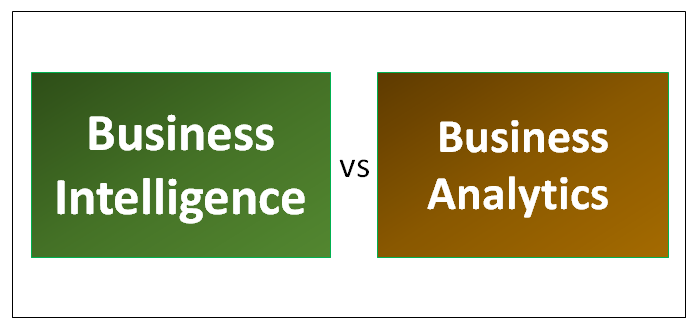
\includegraphics[width=10cm]{./Imagenes/bivsba}
\end{center}
El software de análisis de negocios es un niño o padre (dependiendo de a quién le pregunte) de la categoría de inteligencia empresarial. Al igual que BI, se utiliza principalmente para analizar datos históricos, pero con la intención de predecir las tendencias de negocios. Por lo general, también tiene un ojo hacia la mejora y la preparación para el cambio. 

\end{document}